\documentclass[12pt, a4paper]{report}

\usepackage{amsmath,amsthm,amssymb}
\usepackage{mathtext}
\usepackage[T1,T2A]{fontenc}
\usepackage[utf8]{inputenc}
\usepackage[english,russian]{babel}
\usepackage{listings}
\usepackage{graphicx}
\usepackage{tablefootnote}
\usepackage{indentfirst}
\usepackage{color}
\usepackage{float}
\usepackage{caption}
\captionsetup[table]{singlelinecheck=off}
\captionsetup[lstlisting]{singlelinecheck=off, labelformat=empty}
\usepackage{pgfplots}
\pgfplotsset{compat=1.9}
\usepackage[left=3cm,right=1cm,top=2cm,bottom=2cm,bindingoffset=0cm]{geometry}
\graphicspath{{./img/}}

% Настройка заголовков
\makeatletter
\renewcommand\LARGE{\@setfontsize\LARGE{20pt}{30}}
\renewcommand\Large{\@setfontsize\Large{16pt}{20}}
\renewcommand\large{\@setfontsize\large{14pt}{20}}
\makeatother
\RequirePackage{titlesec}
\titleformat{\chapter}{\LARGE\bfseries}{\thechapter}{14pt}{\LARGE\bfseries}
\titleformat{\section}{\Large\bfseries}{\thesection}{14pt}{\Large\bfseries}
\titleformat{\sub}{\large\bfseries}{\thesubsection}{14pt}{\large\bfseries}
\titlespacing{\chapter}{12.5mm}{-22pt}{40pt}
\titlespacing{\section}{12.5mm}{20pt}{20pt}
\titlespacing{\subsection}{12.5mm}{10pt}{10pt}

\lstset{ 
	backgroundcolor=\color{white},   % choose the background color; you must add \usepackage{color} or \usepackage{xcolor}
	breaklines=true,                 % sets automatic line breaking
	captionpos=t,                    % sets the caption-position to bottom
	commentstyle=\color{green},    % comment style
	keywordstyle=\color{blue},       % keyword style
	language=C++,                 % the language of the code
	numbers=left,                    % where to put the line-numbers; (none, left, right)
	numbersep=5pt,                   % how far the line-numbers are from the code
	numberstyle=\small\color{black}, % the style that is used for the line-numbers
	showspaces=false,                % show spaces everywhere adding particular underscores; it overrides 'showstringspaces'
	showstringspaces=false,          % underline spaces within strings only
	showtabs=false,                  % show tabs within strings adding particular underscores
	stepnumber=1,                    % the step between two line-numbers. If it's 1, each line will be numbered
	stringstyle=\color{yellow},     % string literal style
	tabsize=2,	                   % sets default tabsize to 2 spaces
	frame=single
}

\begin{document}
	
	\begin{titlepage}
		\noindent \begin{minipage}{0.15\textwidth}
			
\includegraphics[width=\linewidth]{bauman_image}
		\end{minipage}
		\footnotesize\noindent \begin{minipage}{0.8\textwidth}\centering
			\textbf{Министерство науки и высшего образования Российской Федерации}\\
			\textbf{Федеральное государственное бюджетное образовательное учреждение}\\
			\textbf{высшего образования}\\
			\textbf{~~~«Московский государственный технический университет}\\
			\textbf{имени Н.Э.~Баумана}\\
			\textbf{(национальный исследовательский университет)»}\\
			\textbf{(МГТУ им. Н.Э.~Баумана)}
		\end{minipage}
		
		\noindent\rule{17cm}{3pt}
		\newline\newline
		\large\noindent ФАКУЛЬТЕТ $\underline{\text{Информатика и системы управления}}$ \newline\newline
		\noindent КАФЕДРА $\underline{\text{Программное обеспечение ЭВМ и информационные технологии}}$\newline\newline\newline\newline\newline
		
		
		\begin{center}
			\noindent
			\LARGE\textbf{Отчёт по лабораторной работе №5}\newline
			\textbf{по дисциплине "Анализ алгоритмов"}\newline\newline
		\end{center}
		
		\large\noindent\textbf{Тема} $\underline{\text{Конвейерная обработка данных}}$\newline\newline
		\noindent\textbf{Студент} $\underline{\text{Жабин Д.В.}}$\newline\newline
		\noindent\textbf{Группа} $\underline{\text{ИУ7-54Б}}$\newline\newline
		\noindent\textbf{Преподаватель} $\underline{\text{Волкова Л.Л.}}$\newline\newline\newline
		
		\begin{center}
			\large\vfill
			Москва, 2021 г.
		\end{center}
	\end{titlepage}
	
	\setlength{\parindent}{1.25cm}
	
	\renewcommand*\contentsname{Содержание}
	
	\setcounter{page}{2}\large\linespread{1.3}\tableofcontents
	
	\newpage
	\chapter*{Введение}
	\addcontentsline{toc}{chapter}{Введение}
	
	Конвейер~--- способ организации вычислений, используемый в современных процессорах и контроллерах с целью повышения их производительности (увеличения числа инструкций, выполняемых в единицу времени~--- эксплуатация параллелизма на уровне инструкций), технология, используемая при разработке компьютеров и других цифровых электронных устройств.
	
	Идея заключается в параллельном выполнении нескольких инструкций процессора. Сложные инструкции процессора представляются в виде последовательности более простых стадий. Вместо выполнения инструкций последовательно (ожидания завершения конца одной инструкции и перехода к следующей), следующая инструкция может выполняться через несколько стадий выполнения первой инструкции. Это позволяет управляющим цепям процессора получать инструкции со скоростью самой медленной стадии обработки, однако при этом намного быстрее, чем при выполнении эксклюзивной полной обработки каждой инструкции от начала до конца. 
	
	Целью лабораторной работы является получение навыка организации асинхронной передачи данных между потоками на примере конвейера. Для ее достижения поставлены следующие задачи:
	
	\begin{itemize}
		\item выбрать логический алгоритм, выполняющий последовательные преобразования исходных данных;
		\item изучить строение конвейера;
		\item разработать схему реализации конвейерной системы;
		\item реализовать параллельный и последовательный конвейеры;
		\item провести тестирование разработанного программного обеспечения;
		\item провести анализ скорости работы реализаций конвейеров.
	\end{itemize}
	
	\newpage
	\chapter*{1 Аналитическая часть}
	\addcontentsline{toc}{chapter}{1 Аналитическая часть}
	
	Рассмотрим алгоритм нахождения обратной матрицы размером $3\times3$. Обратная матрица может быть найдена, если ее определитель не равен 0 (1.1). Определитель матрицы $A$ размером $3\times3$ можно вычислить по формуле разложения по первой строке (1.2).
	
	$$det \neq 0\eqno (1.1)$$
	
	$$\begin{vmatrix} A_{00}& A_{01}& A_{02}\\ A_{10}& A_{11}& A_{12}\\ A_{20}& A_{21}& A_{22} \end{vmatrix} = A_{00} * \begin{vmatrix} A_{11}& A_{12}\\ A_{21}& A_{22} \end{vmatrix} - A_{01} * \begin{vmatrix} A_{10}& A_{12}\\ A_{20}& A_{22} \end{vmatrix} + A_{02} * \begin{vmatrix} A_{10}& A_{11}\\ A_{20}& A_{21} \end{vmatrix} =$$
	$$A_{00} * (A_{11} * A_{22} - A_{12} * A_{21}) - A_{01} * (A_{10} * A_{22} - A_{12} * A_{20}) + \eqno (1.2)$$
	$$+ A_{02} * (A_{10} * A_{21} - A_{11} * A_{20})$$\newline
	
	Общую формулу нахождения матрицы $A^{-1}$, обратной к матрице $A$, представим как произведение транспонированной матрицы алгебраических дополнений $A_{*}^{T}$ на число, обратное определителю исходной матрицы [4] (1.3).
	$$A^{-1} = \frac{1}{det}A_{*}^{T}\eqno (1.3)$$
	
	Разобьем алгоритм на 3 этапа преобразования исходной матрицы.
	
	\section*{1.1 Нахождение матрицы алгебраических дополнений}
	\addcontentsline{toc}{section}{1.1 Нахождение матрицы алгебраических дополнений}
	
	Матрица алгебраических дополнений состоит из определителей матриц размером $2\times2$. Они получаются путем мысленного вычеркивания столбца и строки элемента, к которому в данный момент считается алгебраическое дополнение. Пример вычисления алгебраического дополнения $A_{*00}$ (1.4), $A_{*01}$ (1.5).
	$$A_{*00} = \begin{vmatrix} A_{11}& A_{12}\\ A_{21}& A_{22} \end{vmatrix} \eqno (1.4)$$
	
	$$A_{*01} = - \begin{vmatrix} A_{10}& A_{12}\\ A_{20}& A_{22} \end{vmatrix} \eqno (1.5)$$\newline
	При этом значение будет взято с обратным знаком в том случае, когда сумма индексов элемента нечетна.
	
	\section*{1.2 Транспонирование матрицы}
	\addcontentsline{toc}{section}{1.2 Транспонирование матрицы}
	
	При транспонировании строки становятся соответствующими столбцами, а столбцы --- строками. Так, при размере матрицы $3\times3$ элементы $A_{01}$ и $A_{10}$, $A_{02}$ и $A_{20}$, $A_{12}$ и $A_{21}$ меняются местами.
	
	\section*{1.3 Умножение матрицы на число}
	\addcontentsline{toc}{section}{1.3 Умножение матрицы на число}
	
	При умножении матрицы на число каждый элемент матрицы умножается на это число.
	
	\section*{1.4 Организация конвейерной системы}
	\addcontentsline{toc}{section}{1.4 Организация конвейерной системы}
	
	Конвейер будет состоять из 4 уровней. Обработанные данные передаются с одного уровня (ленты) конвейера на следующий. На каждой ленте осуществляется обработка данных. Для каждой ленты существует своя очередь необработанных заявок. После обработки на последней ленте конвейера заявки поступают в результирующую очередь. Уровни конвейера:
	\begin{enumerate}
		\item 0 уровень~--- генерация входных данных в первую очередь.
		\item 1 уровень~--- преобразование исходной матрицы к матрице алгебраических дополнений.
		\item 2 уровень~--- транспонирование матрицы алгебраических дополнений.
		\item 3 уровень~--- умножение полученной матрицы на число, обратное определителю исходной матрицы.
	\end{enumerate}
	
	\section*{1.5 Вывод по аналитической части}
	\addcontentsline{toc}{section}{1.5 Вывод по аналитической части}
	В данном разделе была рассмотрена последовательность действий при нахождении обратной матрицы размером $3\times3$, а также описана структура конвейерной системы, с помощью которой можно решить данную задачу.
	
	\newpage
	\chapter*{2 Конструкторская часть}
	\addcontentsline{toc}{chapter}{2 Конструкторская часть}
	
	На основе полученных аналитических данных представим схему работы конвейера, опишем используемые типы и структуры данных, разработаем тесты для проверки корректности работы программы.
	
	\section*{2.1 Схемы алгоритмов}
	\addcontentsline{toc}{section}{2.1 Схемы алгоритмов}
	
	На рисунках 2.1 -- 2.3 представлены схемы алгоритмов работы конвейера и ленты.
	
	\begin{figure}[H]
		\center{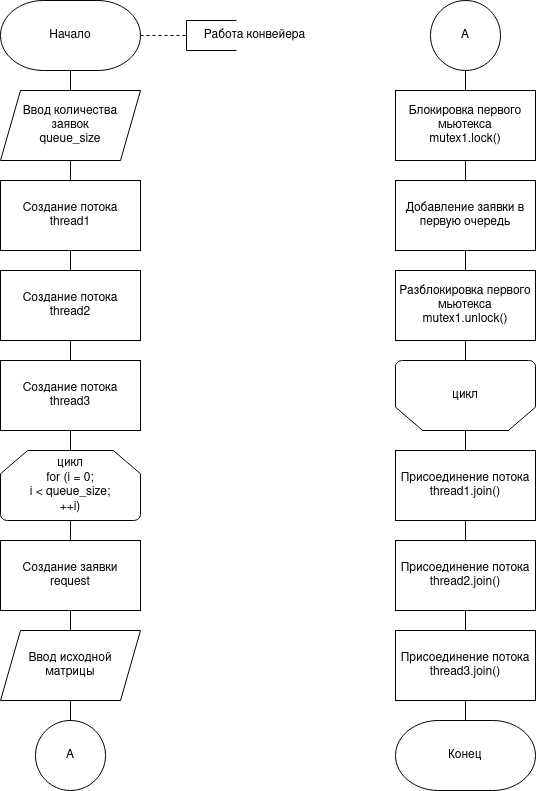
\includegraphics[scale=0.72]{conv.png}}
		\caption*{Рисунок 2.1~--- Алгоритм работы конвейера}
	\end{figure}
	
	\begin{figure}[H]
		\center{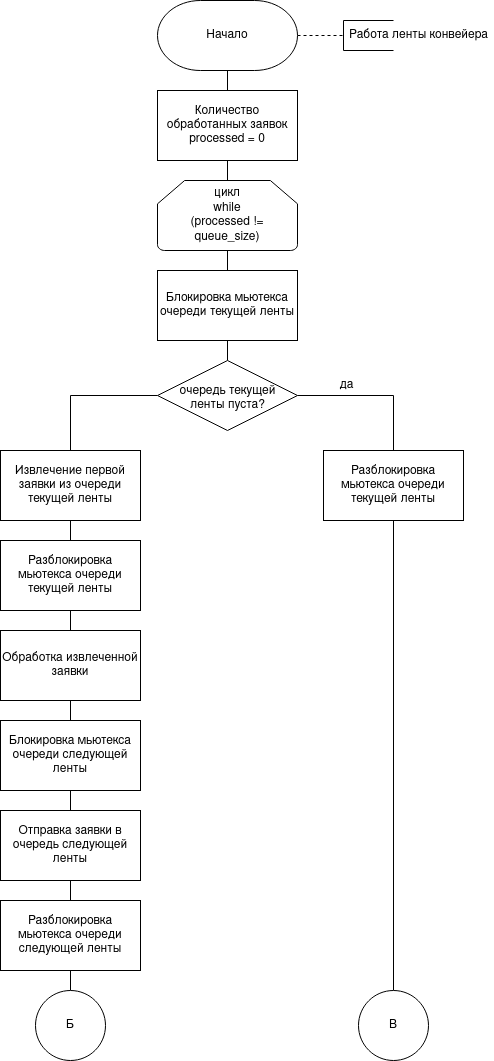
\includegraphics[scale=0.65]{lenta1.png}}
		\caption*{Рисунок 2.2~--- Алгоритм работы ленты конвейера. Часть 1}
	\end{figure}
	
	\begin{figure}[H]
		\center{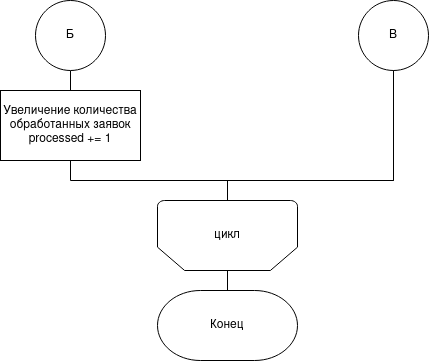
\includegraphics[scale=0.72]{lenta2.png}}
		\caption*{Рисунок 2.3~--- Алгоритм работы ленты конвейера. Часть 2}
	\end{figure}
	
	\section*{2.2 Типы и структуры данных}
	\addcontentsline{toc}{section}{2.2 Типы и структуры данных}
	
	Для реализации очередей линий конвейера используется встроенный тип данных \verb|queue|. Этот тип данных позволяет работать с контейнером, как с очередью, при этом имеет достаточный интерфейс.
	
	Для реализации мьютексов используется встроенный тип данных \verb|mutex|, предоставляющий полный функционал для работы с мьютексами.
	
	Для реализации потоков используется тип данных \verb|thread|, позволяющий создавать потоки, которые могут параллельно выполнять определенные задачи.
	
	Для реализации заявок используется тип данных \verb|request|. Память под матрицу выделяется динамически. Матрица~--- это массив (размером 3) элементов типа указатель на массив (размером 3) типа \verb|float|. Такое хранение матрицы позволяет легко, используя двойные квадратные скобки, получать доступ к любому элементу матрицы. Для заявки хранятся значения времени начала и конца обработки на каждой линии: \verb|in_line[1..3]|~--- момент времени начала обработки заявки, \verb|out_line[1..3]|~--- момент времени конца обработки заявки. Также класс должен содержать такие методы для обработки заявки, как деление матрицы на определитель, вычисление матрицы алгебраических дополнений, транспонирование матрицы.
	
	\section*{2.3 Способ тестирования}
	\addcontentsline{toc}{section}{2.3 Способ тестирования}
	
	Создаваемое программное обеспечение будет протестировано методом \verb|черного ящика|. Для тестирования были выделены следующие классы эквивалентности:
	\begin{enumerate}
		\item Неверный выбор режима работы программы~--- пустой ввод, нецифровой символ или вещественное число.
		\item Верный выбор режима работы программы~--- цифра из диапазона $[1..5]$ или число, выходящее за пределы указанного диапазона.
		\item Неверный ввод количества исходных матриц~--- пустой ввод, нецифровой символ, целое неположительное или вещественное число.
		\item Верный ввод количества исходных матриц~--- целое положительное число.
		\item Неверный ввод элемента исходной матрицы~--- пустой ввод, нецифровой символ или вещественное число.
		\item Верный ввод элемента исходной матрицы~--- целое число.
	\end{enumerate}
	\newpage
	\section*{2.4 Тестовые данные}
	\addcontentsline{toc}{section}{2.4 Тестовые данные}
	
	В таблицах 2.1 -- 2.3 представлены тестовые данные.
	
	\begin{table} [H]
		\caption*{Таблица 2.1~--- Функциональные тесты выбора режима работы программы}
		\begin{tabular}[l]{|c c c|}
			\hline
			Номер тестового случая & Ввод & Ожидаемый результат  \\
			
			1 & \verb|_|\tablefootnote[1]{Пустой ввод} & Неверный ввод \\\hline 
			
			2 & $\alpha$ & Неверный ввод \\\hline
			
			3 & 3.14 & Неверный ввод \\\hline
			
			4 & 1 & Введите элементы матрицы \\\hline 
			
			5 & 2 & Введите элементы матрицы \\\hline 
			
			6 & 3 & Введите количество матриц \\\hline
			
			7 & 4 & Введите количество матриц \\\hline
			
			8 & 5 & Таблица замеров времени \\\hline
			
			9 & 0 & $.$\tablefootnote[2]{Конец работы программы} \\\hline
		\end{tabular}
	\end{table}
	
	\begin{table} [H]
		\caption*{Таблица 2.2~--- Функциональные тесты ввода количества исходных матриц}
		\begin{tabular}[l]{|c c c|}
			\hline
			Номер тестового случая & Ввод & Ожидаемый результат  \\
			
			1 & $\verb|_|^1$ & Неверный ввод \\\hline 
			
			2 & $\alpha$ & Неверный ввод \\\hline 
			
			3 & 0 & Неверный ввод \\\hline 
			
			4 & 3.14 & Неверный ввод \\\hline
			
			5 & 2 & Введите элементы матрицы \\\hline
		\end{tabular}
	\end{table}
	
	\begin{table} [H]
		\caption*{Таблица 2.3~--- Функциональные тесты ввода элементов исходной матрицы}
		\begin{tabular}[l]{|c c c|}
			\hline
			Номер тестового случая & Ввод & Ожидаемый результат  \\
			
			1 & $\verb|_|^1$ & Неверный ввод \\\hline 
			
			2 & $\alpha$ & Неверный ввод \\\hline 
			
			3 & 2.2 & Неверный ввод \\\hline
			
			4 & 0 & $...$\tablefootnote[3]{Ожидание ввода следующего элемента} \\\hline 
		\end{tabular}
	\end{table}
	
	\section*{2.5 Структура программного обеспечения}
	\addcontentsline{toc}{section}{2.5 Структура программного обеспечения}
	
	Программное обеспечение разработано с использованием объектно-\newlineориентированного подхода. Программа содержит функции, отвечающие за линии последовательного \verb|line[1..3]Order| и параллельного \verb|line[1..3]| конвейеров. Они ничего не принимают на вход и ничего не возвращают. Методы класса \verb|request|~--- \verb|setToCofactor|, \verb|setToTranspose|, \verb|divideByDet|~--- ничего не принимают на вход, а лишь изменяют матрицу той заявки, для которой этот метод был вызван.
	
	\section*{2.6 Вывод по конструкторской части}
	\addcontentsline{toc}{section}{2.6 Вывод по конструкторской части}
	
	В данном разделе были разработаны схемы алгоритмов работы конвейера и лент конвейера, а также подготовлены тестовые данные для программного обеспечения. 
	
	\chapter*{3 Технологическая часть}
	\addcontentsline{toc}{chapter}{3 Технологическая часть}
	
	В данном разделе приведены средства реализации и листинги кода, а также перечислены требования к разрабатываемому программному обеспечению.
	
	\section*{3.1 Требования к ПО}
	\addcontentsline{toc}{section}{3.1 Требования к ПО}
	
	К программе предъявляется ряд требований:
	
	\begin{itemize}
		\item требования ко вводу
		\begin{itemize}
			\item должен быть выбран режим работы программы (целое число в диапазоне $[1..5]$);
			\item должны быть введены следующие значения: количество исходных матриц для преобразования при необходимости (целое положительное число), элементы матрицы (целые числа).
		\end{itemize}
		\item требования к выводу
		\begin{itemize}
			\item вычисленные обратные матрицы;
			\item таблица времен работы реализаций конвейеров на случайных значениях в наносекундах.
		\end{itemize}
		\item ограничения работы программы
		\begin{itemize}
			\item при вводе режима работы программы, выходящего за пределы указанного диапазона, программа завершает работу.
		\end{itemize}
		\item функциональные требования к программному обеспечению
		\begin{itemize}
			\item при запуске программа должна выводить меню с возможными режимами работы;
			\item программа должна находить одну или несколько обратных матриц с помощью последовательного или параллельного конвейера;
			\item в исследовательском режиме программа должна замерять время обработки всех запросов последовательным и параллельным конвейером при случайных элементах матриц.
		\end{itemize}
	\end{itemize}
	
	\section*{3.2 Средства реализации}
	\addcontentsline{toc}{section}{3.2 Средства реализации}
	
	Для реализации ПО был выбран язык программирования \verb|С++| [1]. Это обусловлено наличием широкого спектра возможностей для работы с потоками и мьютексами, а такде поддержкой объектно-ориентированного подхода программирования.
	
	В качестве среды разработки была выбрана \verb|Visual Studio Code| [3]. Достаточный опыт работы в этой среде, удобства написания кода и его автодополнения стали ключевыми при выборе.
	
	\section*{3.3 Реализация алгоритмов}
	\addcontentsline{toc}{section}{3.3 Реализация алгоритмов}
	
	В листингах 3.1 -- 3.11 приведены реализации функций, использовавшихся в программном обеспечении.
	
	\newpage
	\begin{lstlisting}[title=Листинг 3.1~--- Функция преобразования матрицы к матрице алгебраических дополнений]
		void request::setToCofactor() {
			float temp1 = values[1][1]*values[2][2] -\
			values[1][2]*values[2][1];
			float temp2 = -(values[1][0]*values[2][2] -\
			values[1][2]*values[2][0]);
			float temp3 = values[1][0]*values[2][1] -\
			values[1][1]*values[2][0];
			float temp4 = -(values[0][1]*values[2][2] -\
			values[0][2]*values[2][1]);
			float temp5 = values[0][0]*values[2][2] -\
			values[0][2]*values[2][0];
			float temp6 = -(values[0][0]*values[2][1] -
			values[0][1]*values[2][0]);
			values[2][0] = values[0][1]*values[1][2] -\
			values[0][2]*values[1][1];
			values[2][1] = -(values[0][0]*values[1][2] -\
			values[0][2]*values[1][0]);
			values[2][2] = values[0][0]*values[1][1] -\
			values[0][1]*values[1][0];
			values[0][0] = temp1;
			values[0][1] = temp2;
			values[0][2] = temp3;
			values[1][0] = temp4;
			values[1][1] = temp5;
			values[1][2] = temp6;
		}
	\end{lstlisting}
	
	\begin{lstlisting}[title=Листинг 3.2~--- Функция транспонирования матрицы]
		void request::setToTranspose() {
			float temp = values[0][1];
			values[0][1] = values[1][0];
			values[1][0] = temp;
			temp = values[0][2];
			values[0][2] = values[2][0];
			values[2][0] = temp;
			temp = values[1][2];
			values[1][2] = values[2][1];
			values[2][1] = temp;
		}
	\end{lstlisting}
	
	\begin{lstlisting}[title=Листинг 3.3~--- {Функция деления матрицы на определитель исходной матрицы}]
		void request::divideByDet() {
			for (int i = 0; i < 3; ++i) {
				for (int j = 0; j < 3; ++j) {
					if (fabs(det) < EPS)
					values[i][j] = 0;
					else
					values[i][j] /= det;
				}
			}
		}
	\end{lstlisting}
	
	\begin{lstlisting}[title=Листинг 3.4~--- Функция первой ленты параллельного конвейера]
		void line1() {
			int processed = 0;
			while (processed != queue_size) {
				mutex1.lock();
				if (queue1.empty()) {
					mutex1.unlock();
					continue;
				}
				request *temp = queue1.front();
				queue1.pop();
				mutex1.unlock();
				temp->setToCofactor();
				mutex2.lock();
				queue2.push(temp);
				mutex2.unlock();
				processed++;
			}
		}
	\end{lstlisting}
	\newpage
	\begin{lstlisting}[title=Листинг 3.5~--- Функция второй ленты параллельного конвейера]
		void line2() {
			int processed = 0;
			while (processed != queue_size) {
				mutex2.lock();
				if (queue2.empty()) {
					mutex2.unlock();
					continue; }
				request *temp = queue2.front();
				queue2.pop();
				mutex2.unlock();
				temp->setToTranspose();
				mutex3.lock();
				queue3.push(temp);
				mutex3.unlock();
				processed++;
			}
		}
	\end{lstlisting}
	
	\begin{lstlisting}[title=Листинг 3.6~--- Функция третьей ленты параллельного конвейера]
		void line3() {
			int processed = 0;
			while (processed != queue_size) {
				mutex3.lock();
				if (queue3.empty()) {
					mutex3.unlock();
					continue;
				}
				request *temp = queue3.front();
				queue3.pop();
				mutex3.unlock();
				temp->divideByDet();
				queue4.push(temp);
				processed++;
			}
		}
	\end{lstlisting}
	\newpage
	\begin{lstlisting}[title=Листинг 3.7~--- Функция первой ленты последовательного конвейера]
		void line1Order() {
			int processed = 0;
			while (processed != queue_size) {
				request *temp = queue1.front();
				queue1.pop();
				temp->setToCofactor();
				queue2.push(temp);
				processed++;
			}
		}
	\end{lstlisting}
	
	\begin{lstlisting}[title=Листинг 3.8~--- Функция второй ленты последовательного конвейера]
		void line2Order() {
			int processed = 0;
			while (processed != queue_size) {
				request *temp = queue2.front();
				queue2.pop();
				temp->setToTranspose();
				queue3.push(temp);
				processed++;
			}
		}
	\end{lstlisting}
	
	\begin{lstlisting}[title=Листинг 3.9~--- Функция третьей ленты последовательного конвейера]
		void line3Order() {
			int processed = 0;
			while (processed != queue_size) {
				request *temp = queue3.front();
				queue3.pop();
				temp->divideByDet();
				queue4.push(temp);
				processed++;
			}
		}
	\end{lstlisting}
	\newpage
	\begin{lstlisting}[title=Листинг 3.10~--- Параллельный конвейер]
		thread thread1(line1);
		thread thread2(line2);
		thread thread3(line3);
		request *temp;
		for (int i = 0; i < queue_size; ++i) {
			temp = new request;
			temp->input();
			mutex1.lock();
			queue1.push(temp);
			mutex1.unlock();
		}
		thread1.join();
		thread2.join();
		thread3.join();
	\end{lstlisting}
	
	\begin{lstlisting}[title=Листинг 3.11~--- Последовательный конвейер]
		request *temp;
		for (int i = 0; i < queue_size; ++i) {
			temp = new request;
			temp->input();
			queue1.push(temp);
		}
		line1();
		line2();
		line3();
	\end{lstlisting}
	\newpage
	\section*{3.4 Пример работы программы}
	\addcontentsline{toc}{section}{3.4 Пример работы программы}
	
	На рисунке (3.1) приведен пример работы программы.
	
	\begin{figure}[H]
		\center{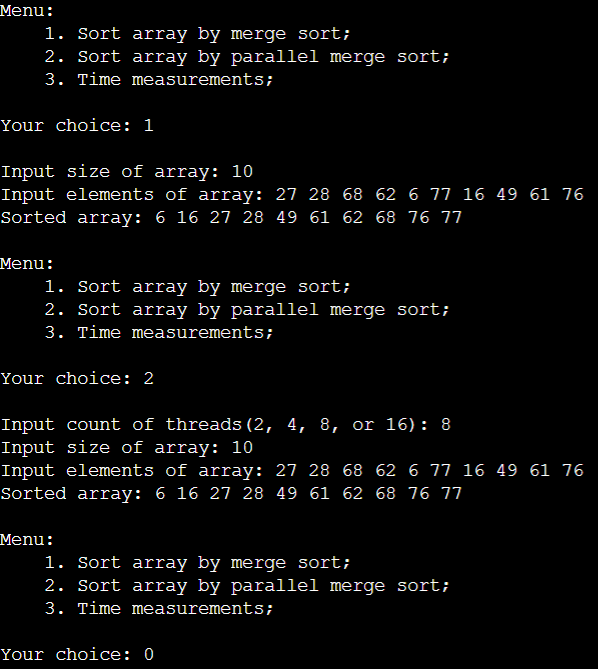
\includegraphics[scale=0.72]{exampleprog.PNG}}
		\caption*{Рисунок 3.1~--- Пример работы программы}
	\end{figure}
	
	\section*{3.5 Вывод по технологической части}
	\addcontentsline{toc}{section}{3.5 Вывод по технологической части}
	
	В данном разделе были описаны средства реализации, представлены требования к ПО и реализованы последовательный и параллельный конвейер для нахождения обратной матрицы.
	
	\chapter*{4 Исследовательская часть}
	\addcontentsline{toc}{chapter}{4 Исследовательская часть}
	
	В этом разделе будет исследовано быстродействие разработанных реализаций конвейеров.
	
	\section*{4.1 Технические характеристики}
	\addcontentsline{toc}{section}{4.1 Технические характеристики}
	
	Ниже приведены технические характеристики устройства, на котором было проведено тестирование ПО:
	
	\begin{itemize}
		\item операционная система Windows 10 64-разрядная;
		\item оперативная память 16 ГБ;
		\item процессор Intel(R) Core(TM) i5-4690 @ 3.50ГГц.
	\end{itemize}
	
	\section*{4.2 Время выполнения реализаций конвейеров}
	\addcontentsline{toc}{section}{4.2 Время выполнения реализаций конвейеров}
	
	Чтобы точно оценить время выполнения реализаций двух конвейеров была использована функция \verb|std::chrono::high_resolution_clock::now()| [2], которая возвращает точку, указывающую на текущее время. Так, с помощью двух последовательных вызовов можно определить, в период какого времени выполнялась функция.
	
	Замеры проводились при длине очереди в 10 заявок.
	
	В таблицах 4.1 и 4.2 приведены результаты замеров. Время в таблицах указано от начала работы параллельного и последовательного конвейера соответственно.
	
	\begin{table} [H]
		\caption*{Таблица 4.1~--- Работа параллельного конвейера (в наносекундах)}
		\begin{tabular}[l]{|c c c c|}
			\hline
			Линия № & Заявка № & Начало обработки & Конец обработки  \\\hline
			
			1 & 1 & 146430 & 147208  \\ 
			
			2 & 1 & 156072 & 156660  \\ 
			
			3 & 1 & 166374 & 167627  \\\hline
			
			1 & 2 & 164384 & 164979  \\ 
			
			2 & 2 & 170763 & 171335  \\ 
			
			3 & 2 & 175956 & 176864  \\\hline
			
			1 & 3 & 169114 & 169666  \\ 
			
			2 & 3 & 177881 & 178291  \\ 
			
			3 & 3 & 182391 & 183223  \\\hline
			
			1 & 4 & 170483 & 171173  \\ 
			
			2 & 4 & 183906 & 184471  \\ 
			
			3 & 4 & 188749 & 189563  \\\hline
			
			1 & 5 & 172411 & 172992  \\ 
			
			2 & 5 & 190423 & 190833  \\ 
			
			3 & 5 & 199256 & 199825  \\\hline
			
			1 & 6 & 173604 & 174066  \\ 
			
			2 & 6 & 192104 & 192340  \\ 
			
			3 & 6 & 203401 & 203771  \\\hline
			
			1 & 7 & 174556 & 175108  \\ 
			
			2 & 7 & 198124 & 198353  \\ 
			
			3 & 7 & 204599 & 204941  \\\hline
			
			1 & 8 & 175881 & 176433  \\ 
			
			2 & 8 & 198864 & 199259  \\ 
			
			3 & 8 & 205389 & 205825  \\\hline
			
			1 & 9 & 177228 & 177764  \\ 
			
			2 & 9 & 199798 & 200200  \\ 
			
			3 & 9 & 206364 & 206916  \\\hline
			
			1 & 10 & 178595 & 179161  \\ 
			
			2 & 10 & 205833 & 206239  \\ 
			
			3 & 10 & 207631 & 208114  \\\hline
		\end{tabular}
	\end{table}
	
	\begin{table} [H]
		\caption*{Таблица 4.2~--- Работа последовательного конвейера (в наносекундах)}
		\begin{tabular}[l]{|c c c c|}
			\hline
			Линия № & Заявка № & Начало обработки & Конец обработки  \\\hline
			
			1 & 1 & 2125 & 2708  \\ 
			
			2 & 1 & 10625 & 10832  \\ 
			
			3 & 1 & 15170 & 15843  \\\hline
			
			1 & 2 & 3144 & 3712  \\ 
			
			2 & 2 & 11145 & 11343  \\ 
			
			3 & 2 & 16088 & 16473  \\\hline
			
			1 & 3 & 4019 & 4603  \\ 
			
			2 & 3 & 11588 & 11777  \\ 
			
			3 & 3 & 16712 & 17005  \\\hline
			
			1 & 4 & 4902 & 5378  \\ 
			
			2 & 4 & 12027 & 12218  \\ 
			
			3 & 4 & 17242 & 17527  \\\hline
			
			1 & 5 & 5685 & 6103  \\ 
			
			2 & 5 & 12457 & 12645  \\ 
			
			3 & 5 & 17753 & 18037  \\\hline
			
			1 & 6 & 6445 & 6856  \\ 
			
			2 & 6 & 12875 & 13069  \\ 
			
			3 & 6 & 18277 & 18559  \\\hline
			
			1 & 7 & 7159 & 7583  \\ 
			
			2 & 7 & 13304 & 13492  \\ 
			
			3 & 7 & 18802 & 19077  \\\hline
			
			1 & 8 & 7860 & 8243  \\ 
			
			2 & 8 & 13721 & 13912  \\ 
			
			3 & 8 & 19315 & 19596  \\\hline
			
			1 & 9 & 8527 & 8934  \\ 
			
			2 & 9 & 14147 & 14337  \\ 
			
			3 & 9 & 19827 & 20106  \\\hline
			
			1 & 10 & 9200 & 9554  \\ 
			
			2 & 10 & 14582 & 14755  \\ 
			
			3 & 10 & 20343 & 20626  \\\hline
		\end{tabular}
	\end{table}
	
	При этом суммарное время работы параллельного конвейера составило 282084 наносекунды, а последовательного~--- 20720 наносекунд.
	
	Для чистоты эксперимента был запущен тест при длине очереди в 50 заявок. Вместо обрабатывающих функций была использована команда\newline \verb|Sleep(100)|, которая имитирует выполнение задачи. При этом были получены следующие результаты: время работы параллельного конвейера составило 116150200 наносекунд, последовательного~--- 326595400 наносекунд, что примерно в 3 раза дольше.
	
	\section*{4.3 Вывод по исследовательской части}
	\addcontentsline{toc}{section}{4.3 Вывод по исследовательской части}
	
	По результатам замеров можно сказать, что сложность задачи, решаемой каждой лентой конвейера, недостаточна для того, чтобы перекрыть расходы на создание потоков, блокировку и разблокировку мьютексов. При большом количестве заявок в очереди, а также достаточно сложной задаче, параллельный конвейер показывает результат лучше, чем последовательный. При несложной задаче и малом количестве заявок последовательный конвейер покажет лучший результат, поскольку в этом случае не нужно создавать потоки, работать с мьютексами.
	
	
	\chapter*{Заключение}
	\addcontentsline{toc}{chapter}{Заключение}
	
	В ходе проделанной работы была достигнута поставленная цель и решены следующие задачи:
	
	\begin{itemize}
		\item изучено строение конвейера;
		\item разработана схема реализации конвейерной системы;
		\item реализованы последовательный и параллельный конвейеры;
		\item проведено тестирование разработанного программного обеспечения;
		\item проведен анализ скорости работы реализаций конвейеров.
	\end{itemize}
	
	Было доказано, что выделять потоки следует только в том случае, если каждому потоку будет дана сложная задача, в противном случае намного больше времени будет затрачиваться на создание потоков. При объемной задаче параллельный конвейер показал результат лучше, чем последовательный, что доказывает целесообразность использования потоков для более быстрого решения больших задач.
	
	\chapter*{Список литературы}
	\addcontentsline{toc}{chapter}{Список литературы}
	
	[1] C++ [Электронный ресурс]. Режим доступа: https://isocpp.org/. Дата обращения: 21.12.2021.\\
	
	[2] Функция now() [Электронный ресурс]. Режим доступа: \newline https://en.cppreference.com/w/cpp/chrono/high-resolution-clock/now. Дата обращения: 21.12.2021.\\
	
	[3] Visual Studio Code - Code Editing [Электронный ресурс]. Режим доступа: https://code.visualstudio.com. Дата обращения: 21.12.2021.\\
	
	[4] Обратная матрица [Электронный ресурс]. Режим доступа: \newline http://www.mathprofi.ru/kak-naiti-obratnuyu-matricu.html. Дата обращения: \newline21.12.2021.
	
\end{document}
